\documentclass[12pt,a4paper]{article}

% -- Packages ------------------------------------------------------------------
\usepackage[utf8]{inputenc}
\usepackage[T1]{fontenc}
\usepackage[margin=2.5cm]{geometry}
\usepackage{amsmath,amssymb}
\usepackage{graphicx}
\usepackage{hyperref}
\usepackage{booktabs}
\usepackage{enumitem}
\usepackage{xcolor}
\usepackage{listings}
\usepackage{algorithm}
\usepackage{algpseudocode}
\usepackage[most]{tcolorbox}
\usepackage{tikz}
\usetikzlibrary{arrows.meta, positioning, shapes.geometric, shapes.multipart, shapes.misc, calc, backgrounds}

% -- tcolorbox styles ----------------------------------------------------------
\tcbset{
  formulabox/.style={
    colback=yellow!10, colframe=orange!60!black,
    fonttitle=\bfseries, title={Formula},
    left=6pt, right=6pt, top=4pt, bottom=4pt
  },
  definitionbox/.style={
    colback=blue!5, colframe=blue!50!black,
    fonttitle=\bfseries, title={Definition},
    left=6pt, right=6pt, top=4pt, bottom=4pt
  },
  notebox/.style={
    colback=green!5, colframe=green!50!black,
    fonttitle=\bfseries, title={Note},
    left=6pt, right=6pt, top=4pt, bottom=4pt
  },
  warningbox/.style={
    colback=red!5, colframe=red!50!black,
    fonttitle=\bfseries, title={Warning},
    left=6pt, right=6pt, top=4pt, bottom=4pt
  },
}

% -- listings style ------------------------------------------------------------
\lstdefinestyle{python}{
  language=Python,
  basicstyle=\ttfamily\small,
  keywordstyle=\color{blue!70!black}\bfseries,
  commentstyle=\color{gray}\itshape,
  stringstyle=\color{orange!70!black},
  numberstyle=\tiny\color{gray},
  numbers=left,
  frame=single,
  framesep=4pt,
  breaklines=true,
  showstringspaces=false,
  tabsize=4,
}
\lstdefinestyle{yaml}{
  basicstyle=\ttfamily\small,
  keywordstyle=\color{purple}\bfseries,
  commentstyle=\color{gray}\itshape,
  stringstyle=\color{green!50!black},
  frame=single,
  breaklines=true,
  showstringspaces=false,
}

% -- Metadata ------------------------------------------------------------------
\title{\textbf{Navigation Package} \\[6pt]
  \large A* Path Planning on Occupancy Grids for ORB-SLAM3 Maps}
\author{ORB-SLAM3 Relocalization Project}
\date{May 2026}

% ==============================================================================
\begin{document}
\maketitle
\tableofcontents
\newpage

% ==============================================================================
\section{Introduction}
% ==============================================================================

The \textbf{navigation package} turns a 3-D ORB-SLAM3 point cloud into a 2-D
occupancy grid and plans collision-free paths across it using A*.
It is designed as a standalone ROS2 Humble Python package that plugs directly
into the rest of the relocalization pipeline: the same map that ORB-SLAM3 uses
for tracking is projected top-down, and the live pose from
\texttt{/relocalization/pose} drives the robot indicator on the map.

The package solves three problems:

\begin{enumerate}[label=\arabic*.]
  \item \textbf{Map building} --- converting sparse 3-D point cloud data
        (exported as a CSV) into a clean 2-D binary occupancy grid.
  \item \textbf{Path planning} --- finding a smooth, obstacle-free path between
        the robot's current position and a user-selected goal using A*.
  \item \textbf{Visualization} --- displaying the grid, the planned path,
        and the robot's trail in real time via a PyQt5 window.
\end{enumerate}

\begin{tcolorbox}[notebox]
  You do \emph{not} need to understand ORB-SLAM3 internals to use this
  package. The only input it needs is a CSV of 3-D map points
  (\texttt{x, y, z} columns) and, optionally, a live
  \texttt{geometry\_msgs/Pose} from the relocalization node.
\end{tcolorbox}

% ==============================================================================
\section{System Architecture}
% ==============================================================================

The package contains three ROS2 nodes that communicate over topics.

\begin{figure}[h]
\centering
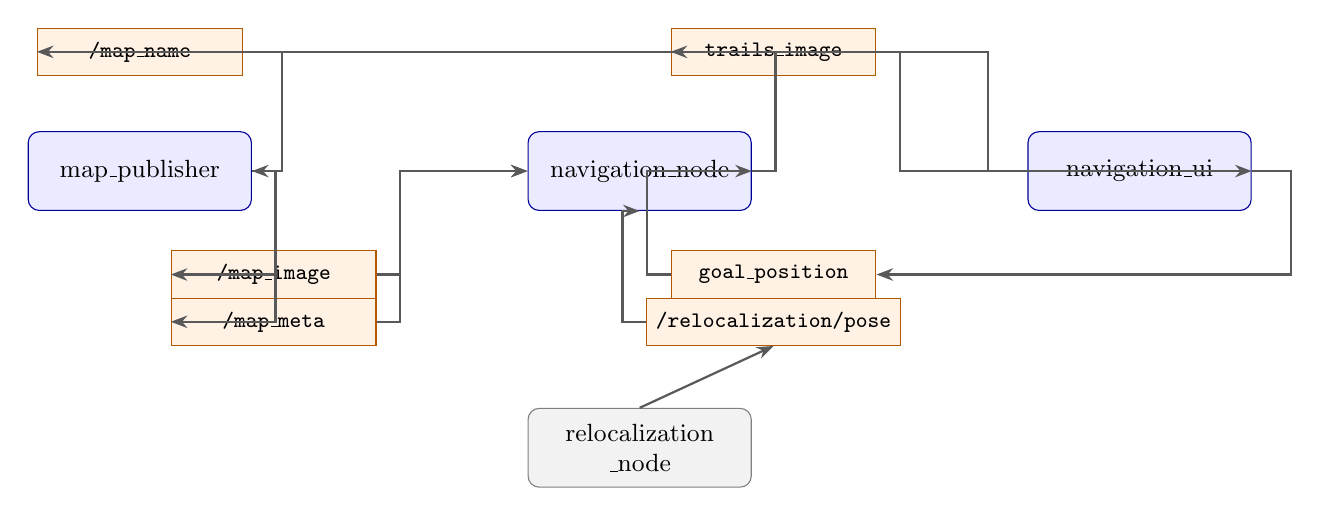
\begin{tikzpicture}[
  node distance = 1.8cm and 2.8cm,
  every node/.style = {font=\small},
  process/.style = {
    rectangle, rounded corners=4pt,
    draw=blue!60!black, fill=blue!8,
    minimum width=2.8cm, minimum height=1cm,
    text centered, text width=2.6cm
  },
  topic/.style = {
    rectangle, draw=orange!70!black, fill=orange!10,
    minimum width=2.6cm, minimum height=0.6cm,
    font=\ttfamily\footnotesize, text centered
  },
  arr/.style = {-{Stealth[length=6pt]}, thick, gray!70!black}
]

% Nodes
\node[process] (mp) {map\_publisher};
\node[process, right=3.5cm of mp] (nav) {navigation\_node};
\node[process, right=3.5cm of nav] (ui) {navigation\_ui};

% Topics between map_publisher and navigation_node
\node[topic, above=0.7cm of mp] (map_name) {/map\_name};
\node[topic, below=0.5cm of mp, xshift=1.7cm] (map_image) {/map\_image};
\node[topic, below=1.1cm of mp, xshift=1.7cm] (map_meta) {/map\_meta};

% Topics from navigation_node to ui
\node[topic, above=0.7cm of nav, xshift=1.7cm] (trails) {trails\_image};

% Topics to navigation_node
\node[topic, below=0.5cm of nav, xshift=1.7cm] (goal) {goal\_position};
\node[topic, below=1.1cm of nav, xshift=1.7cm] (pose) {/relocalization/pose};

% External
\node[process, below=2.5cm of nav, fill=gray!10, draw=gray] (reloc) {relocalization\\\_node};

% Arrows
\draw[arr] (ui.west) -- ++(-0.5,0) |- (map_name.west);
\draw[arr] (map_name.east) -- ++(0.5,0) |- (mp.east);
\draw[arr] (mp.east) -- ++(0.3,0) |- (map_image.west);
\draw[arr] (map_image.east) -- ++(0.3,0) |- (nav.west);
\draw[arr] (mp.east) -- ++(0.3,0) |- (map_meta.west);
\draw[arr] (map_meta.east) -- ++(0.3,0) |- (nav.west);
\draw[arr] (nav.east) -- ++(0.3,0) |- (trails.west);
\draw[arr] (trails.east) -- ++(0.3,0) |- (ui.east);
\draw[arr] (ui.east) -- ++(0.5,0) |- (goal.east);
\draw[arr] (goal.west) -- ++(-0.3,0) |- (nav.east);
\draw[arr] (reloc.north) -- (pose.south);
\draw[arr] (pose.west) -- ++(-0.3,0) |- (nav.south);

\end{tikzpicture}
\caption{ROS2 topic graph of the navigation package. Arrows show data flow direction.}
\label{fig:ros_graph}
\end{figure}

\subsection{Node Roles}

\begin{center}
\begin{tabular}{lll}
\toprule
\textbf{Node} & \textbf{Executable} & \textbf{Role} \\
\midrule
\texttt{map\_publisher} & \texttt{ros2 run navigation map\_publisher} & Loads CSV/PNG map, publishes grid at 1~Hz \\
\texttt{navigation\_node} & \texttt{ros2 run navigation navigation} & A* planning, deviation check, visualization \\
\texttt{navigation\_ui} & \texttt{ros2 run navigation navigation\_ui} & PyQt5 window, goal clicks, map selector \\
\bottomrule
\end{tabular}
\end{center}

% ==============================================================================
\section{Occupancy Grid Construction}
% ==============================================================================

An \textbf{occupancy grid} is a 2-D array where each cell holds a binary
value: \(1\) (occupied / wall) or \(0\) (free / traversable).
The \texttt{map\_publisher} node builds this grid from a CSV of 3-D map points
exported from ORB-SLAM3.

\subsection{Pipeline Overview}

\begin{center}
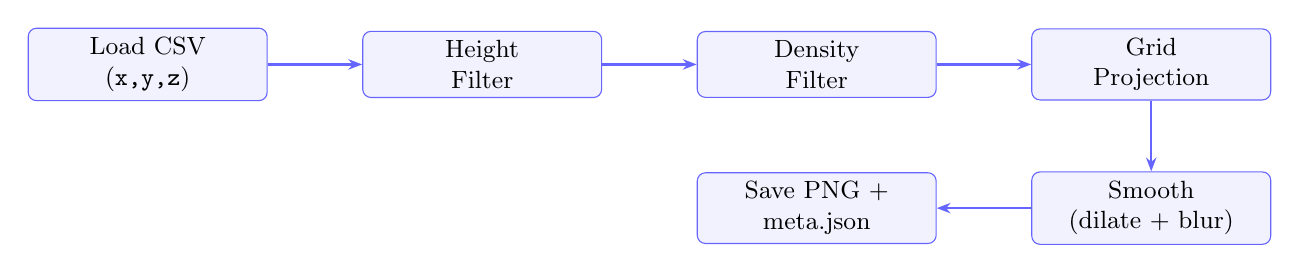
\begin{tikzpicture}[
  box/.style={rectangle, rounded corners=3pt, draw=blue!60, fill=blue!5,
              minimum width=3cm, minimum height=0.7cm, text centered,
              font=\small, text width=2.8cm},
  arr/.style={-{Stealth[length=5pt]}, thick, blue!60}
]
\node[box] (csv)    {Load CSV\\(\texttt{x,y,z})};
\node[box, right=1.2cm of csv] (hf) {Height\\Filter};
\node[box, right=1.2cm of hf]  (df) {Density\\Filter};
\node[box, right=1.2cm of df]  (gp) {Grid\\Projection};
\node[box, below=0.9cm of gp]  (sm) {Smooth\\(dilate + blur)};
\node[box, left=1.2cm of sm]   (save) {Save PNG +\\meta.json};

\draw[arr] (csv) -- (hf);
\draw[arr] (hf)  -- (df);
\draw[arr] (df)  -- (gp);
\draw[arr] (gp)  -- (sm);
\draw[arr] (sm)  -- (save);
\end{tikzpicture}
\end{center}

\subsection{Step 1 --- Height Filter}

ORB-SLAM3 maps contain points at all heights: floor, walls, ceiling, furniture.
For 2-D navigation we keep only points near the ``waist'' of the scene.

\begin{tcolorbox}[formulabox, title={Height Filter}]
Let $\mu_y$ and $\sigma_y$ be the mean and standard deviation of all
$y$-coordinates (vertical axis in ORB-SLAM3 convention). Keep point $p$ if:
\[
  \mu_y - \sigma_y < p_y < \mu_y + \sigma_y
\]
This removes floor and ceiling points while keeping the bulk of wall structure.
\end{tcolorbox}

\subsection{Step 2 --- Density Filter}

Sparse ``stray'' points from reflections or tracking errors are removed using a
neighbourhood count:

\begin{tcolorbox}[formulabox, title={Density Filter}]
Build a BallTree over the $(x, z)$ projections. Keep point $p$ if:
\[
  |\{q \mid \|q_{xz} - p_{xz}\| < 0.3~\text{m}\}| \geq 3
\]
Points with fewer than 3 neighbours within 30~cm are discarded as outliers.
\end{tcolorbox}

\subsection{Step 3 --- Grid Projection}

The surviving points are projected onto a 2-D grid.
ORB-SLAM3 uses \textbf{right-handed coordinates}: $X$ rightward, $Y$ upward,
$Z$ forward. For top-down navigation we project onto the $X$--$Z$ plane.

\begin{tcolorbox}[formulabox, title={World-to-Grid Conversion}]
Given resolution $r$ (metres per pixel) and minimum world coordinates
$(x_{\min},\, z_{\min})$:
\begin{align}
  \mathrm{col} &= \left\lfloor \frac{x - x_{\min}}{r} \right\rfloor
  \label{eq:col} \\[4pt]
  \mathrm{row} &= \left\lfloor \frac{z - z_{\min}}{r} \right\rfloor
  \label{eq:row}
\end{align}
The default resolution is $r = 0.02$~m/px (50~pixels per metre).
Grid cells that contain at least one projected point are marked 255 (wall).
\end{tcolorbox}

\begin{tcolorbox}[notebox]
  Subtracting $(x_{\min}, z_{\min})$ shifts the coordinate origin to the
  map corner, so pixel $(0,0)$ corresponds to the world minimum, \emph{not}
  the ORB-SLAM3 world origin $(0,0,0)$. This offset is stored in
  \texttt{map.meta.json} and broadcast on \texttt{/map\_meta} so the
  navigation node can convert live poses correctly.
\end{tcolorbox}

\subsection{Step 4 --- Smoothing}

Raw point-cloud grids are noisy. A two-stage smoothing closes small gaps and
merges nearby wall clusters:

\begin{enumerate}
  \item \textbf{Morphological dilation} with a $7{\times}7$ kernel,
        2 iterations --- thickens wall pixels outward.
  \item \textbf{Gaussian blur} ($9{\times}9$, $\sigma=2$) --- blends edges.
  \item \textbf{Re-threshold} at 127 --- restores binary values.
\end{enumerate}

The resulting PNG is saved alongside the CSV and reloaded on subsequent runs,
skipping the expensive CSV pipeline entirely.

% ==============================================================================
\section{Coordinate Systems}
% ==============================================================================

Three coordinate systems appear in this package. Confusing them is the most
common source of bugs.

\begin{figure}[h]
\centering
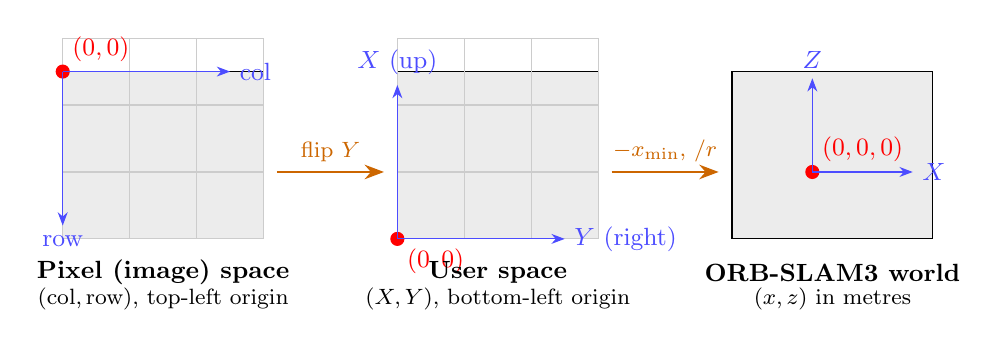
\begin{tikzpicture}[scale=0.85, font=\small]

% -- Pixel coordinate frame -------------------------------------------------
\begin{scope}[xshift=0cm]
  \draw[fill=gray!15] (0,0) rectangle (3,2.5);
  \foreach \c in {0,1,2} \foreach \r in {0,1,2}
    \draw[gray!40] (\c,\r) rectangle (\c+1,\r+1);
  % origin
  \fill[red] (0,2.5) circle (3pt) node[above right, text=red] {$(0,0)$};
  % axes
  \draw[-{Stealth}, blue!70] (0,2.5) -- (2.5,2.5) node[right] {col};
  \draw[-{Stealth}, blue!70] (0,2.5) -- (0,0.2)   node[below] {row};
  \node at (1.5,-0.5) {\textbf{Pixel (image) space}};
  \node[font=\footnotesize] at (1.5,-0.9) {$(\text{col}, \text{row})$, top-left origin};
\end{scope}

% -- User coordinate frame --------------------------------------------------
\begin{scope}[xshift=5cm]
  \draw[fill=gray!15] (0,0) rectangle (3,2.5);
  \foreach \c in {0,1,2} \foreach \r in {0,1,2}
    \draw[gray!40] (\c,\r) rectangle (\c+1,\r+1);
  % origin
  \fill[red] (0,0) circle (3pt) node[below right, text=red] {$(0,0)$};
  % axes
  \draw[-{Stealth}, blue!70] (0,0) -- (2.5,0) node[right] {$Y$ (right)};
  \draw[-{Stealth}, blue!70] (0,0) -- (0,2.3) node[above] {$X$ (up)};
  \node at (1.5,-0.5) {\textbf{User space}};
  \node[font=\footnotesize] at (1.5,-0.9) {$(X, Y)$, bottom-left origin};
\end{scope}

% -- World coordinate frame -------------------------------------------------
\begin{scope}[xshift=10cm]
  \draw[fill=gray!15] (0,0) rectangle (3,2.5);
  % origin
  \fill[red] (1.2,1.0) circle (3pt) node[above right, text=red] {$(0,0,0)$};
  \draw[-{Stealth}, blue!70] (1.2,1.0) -- (2.7,1.0) node[right] {$X$};
  \draw[-{Stealth}, blue!70] (1.2,1.0) -- (1.2,2.4) node[above] {$Z$};
  \node at (1.5,-0.5) {\textbf{ORB-SLAM3 world}};
  \node[font=\footnotesize] at (1.5,-0.9) {$(x, z)$ in metres};
\end{scope}

% -- Conversion arrows ------------------------------------------------------
\draw[-{Stealth[length=7pt]}, thick, orange!80!black]
  (3.2, 1.0) -- (4.8, 1.0) node[midway, above, font=\footnotesize] {flip $Y$};

\draw[-{Stealth[length=7pt]}, thick, orange!80!black]
  (8.2, 1.0) -- (9.8, 1.0)
  node[midway, above, font=\footnotesize] {$-x_{\min}$, $/r$};

\end{tikzpicture}
\caption{The three coordinate systems. The navigation node converts
  \emph{into} pixel space for all internal computation.}
\label{fig:coords}
\end{figure}

\subsection{Conversions}

Let $H$ be the grid height in pixels and $r = 0.02$~m/px.

\begin{tcolorbox}[formulabox, title={User Space $\to$ Pixel Space}]
The UI publishes goals in user space $(X_u, Y_u)$ with origin at
bottom-left, $X$ upward:
\begin{align}
  \mathrm{col} &= Y_u \\
  \mathrm{row} &= H - 1 - X_u
\end{align}
\end{tcolorbox}

\begin{tcolorbox}[formulabox, title={ORB-SLAM3 World $\to$ Pixel Space}]
The relocalization node publishes \texttt{geometry\_msgs/Pose} with
position $(p_x, p_y, p_z)$ in ORB-SLAM3 world metres:
\begin{align}
  \mathrm{col} &= \left\lfloor \frac{p_x - x_{\min}}{r} \right\rfloor \\
  \mathrm{row} &= H - 1 - \left\lfloor \frac{p_z - z_{\min}}{r} \right\rfloor
\end{align}
The subtraction of $(x_{\min}, z_{\min})$ is essential: without it, the
robot at world position $(0,0)$ would be placed at a pixel far outside the
actual map extent.
\end{tcolorbox}

\begin{tcolorbox}[notebox]
  The row formula contains $H - 1 - \cdots$ because increasing $Z$
  (moving forward in ORB-SLAM3) should move the robot \emph{upward} on
  screen. Image rows increase downward, so we invert the row index.
\end{tcolorbox}

% ==============================================================================
\section{Obstacle Inflation}
% ==============================================================================

A robot is not a point --- it has physical width. Even if the robot centre
follows a path that technically avoids obstacles, the robot body may still
collide with a wall. \textbf{Obstacle inflation} solves this by expanding
every obstacle cell outward before planning, so the planner treats the robot
as a point but the inflated walls already include a safety margin.

\begin{figure}[h]
\centering
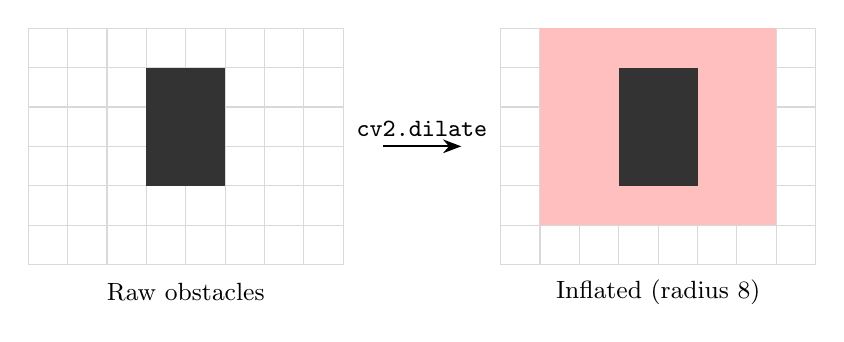
\begin{tikzpicture}[scale=0.5]
  % Raw grid
  \begin{scope}
    \foreach \c in {0,...,7} \foreach \r in {0,...,5}
      \draw[gray!30] (\c,\r) rectangle (\c+1,\r+1);
    % wall cells
    \foreach \pos in {(3,2),(3,3),(3,4),(4,2),(4,3),(4,4)}
      \fill[black!80] \pos rectangle ++(1,1);
    \node at (4,-0.7) {\small Raw obstacles};
  \end{scope}

  \draw[-{Stealth}, thick] (9,3) -- (11,3)
    node[midway, above, font=\small] {\texttt{cv2.dilate}};

  % Inflated grid
  \begin{scope}[xshift=12cm]
    \foreach \c in {0,...,7} \foreach \r in {0,...,5}
      \draw[gray!30] (\c,\r) rectangle (\c+1,\r+1);
    % inflated zone (2px radius)
    \foreach \pos in {%
      (1,1),(2,1),(3,1),(4,1),(5,1),(6,1),%
      (1,2),(2,2),(3,2),(4,2),(5,2),(6,2),%
      (1,3),(2,3),(3,3),(4,3),(5,3),(6,3),%
      (1,4),(2,4),(3,4),(4,4),(5,4),(6,4),%
      (1,5),(2,5),(3,5),(4,5),(5,5),(6,5)}
      \fill[red!25] \pos rectangle ++(1,1);
    % original wall
    \foreach \pos in {(3,2),(3,3),(3,4),(4,2),(4,3),(4,4)}
      \fill[black!80] \pos rectangle ++(1,1);
    \node at (4,-0.7) {\small Inflated (radius 8)};
  \end{scope}
\end{tikzpicture}
\caption{Obstacle inflation: original wall cells (black) are expanded into
  a forbidden zone (red). The planner plans only in white cells.}
\label{fig:inflation}
\end{figure}

\subsection{Implementation}

Inflation is computed \emph{once per map update}, not once per planning call:

\begin{lstlisting}[style=python, caption={Inflation in map\_callback (main.py)}]
# kernel covers all 8 directions equally --- MORPH_RECT preserves corners
kernel = cv2.getStructuringElement(cv2.MORPH_RECT, (2*radius+1, 2*radius+1))
inflated = cv2.dilate(binary_map, kernel, iterations=1)
\end{lstlisting}

\begin{tcolorbox}[notebox]
  \textbf{Why \texttt{MORPH\_RECT} and not \texttt{MORPH\_ELLIPSE}?}
  A rectangular kernel inflates corners diagonally, matching 8-connected
  A* movement. An elliptical kernel leaves diagonal corners exposed, which
  can allow the planner to route through a one-pixel gap at a wall corner.
\end{tcolorbox}

The cached inflated map is reused for every plan call. At plan time, the start
and goal cells are explicitly cleared (set to 0) so they are never treated as
obstacles even if they lie inside the inflation zone.

% ==============================================================================
\section{A* Path Planning}
% ==============================================================================

A* is a best-first graph search algorithm that finds the optimal
(lowest-cost) path between two cells in a grid. It combines the actual cost
to reach a node with an estimate of the remaining cost to the goal.

\subsection{Cost Functions}

\begin{tcolorbox}[definitionbox, title={A* Scores}]
For each grid cell $n$:
\begin{align}
  g(n) &= \text{actual cost from start to } n \label{eq:g}\\
  h(n) &= \text{estimated cost from } n \text{ to goal (heuristic)} \label{eq:h}\\
  f(n) &= g(n) + h(n) \label{eq:f}
\end{align}
A* always expands the open node with the lowest $f$-score.
\end{tcolorbox}

This implementation uses \textbf{Euclidean distance} as the heuristic,
which is admissible (never overestimates) because straight-line distance
is always $\leq$ the true path length:

\begin{tcolorbox}[formulabox, title={Heuristic}]
\[
  h(n) = \sqrt{(n_x - g_x)^2 + (n_y - g_y)^2}
\]
where $(g_x, g_y)$ is the goal cell in pixel coordinates.
\end{tcolorbox}

\textbf{Movement cost.}
The planner allows 8-connected movement (cardinal and diagonal).
Moving diagonally costs $\sqrt{2}$ times a cardinal step to avoid
artificially preferring diagonals:

\begin{tcolorbox}[formulabox, title={Step Cost}]
\[
  c(n, m) =
  \begin{cases}
    1 & \text{if } m \text{ is a cardinal neighbour of } n \\
    \sqrt{2} & \text{if } m \text{ is a diagonal neighbour of } n
  \end{cases}
\]
\[
  g(m) = g(n) + c(n, m)
\]
\end{tcolorbox}

\subsection{Algorithm --- Open List with Lazy Deletion}

The classic A* maintains two sets:
\begin{itemize}
  \item \textbf{Open set} --- nodes discovered but not yet expanded (a priority queue ordered by $f$).
  \item \textbf{Closed set} --- nodes already expanded.
\end{itemize}

A naive open set backed by a list requires $O(n)$ to find and update the
minimum-$f$ entry. This implementation uses a \textbf{binary heap}
(\texttt{heapq}) with \textbf{lazy deletion}:

\begin{tcolorbox}[definitionbox, title={Lazy Deletion}]
  When a node's $g$-cost improves, a \emph{new} heap entry is pushed
  with the updated $f$. The stale entry remains in the heap but is
  \textbf{skipped} at pop time by checking whether the node was already
  visited. This avoids costly $O(n)$ heap updates while keeping
  $O(\log n)$ push and pop.
\end{tcolorbox}

\begin{algorithm}[H]
\caption{A* with Heapq and Lazy Deletion}
\begin{algorithmic}[1]
\State Push $(f_{\text{start}},\; \text{counter},\; \text{start})$ onto heap; $g[\text{start}] \gets 0$
\While{heap is not empty \textbf{and} iterations $< $ limit}
  \State $(\_,\; \_,\; n) \gets$ \textsc{Pop}(heap)
  \If{$n \in \text{visited}$} \textbf{continue} \Comment{lazy deletion --- stale entry}
  \EndIf
  \State Add $n$ to visited
  \If{$\|n - \text{goal}\| \leq 1.5$ \textbf{and} line-of-sight to goal is clear}
    \State $\text{goal.parent} \gets n$; \textbf{break}
  \EndIf
  \For{each free neighbour $m$ of $n$}
    \State $g_{\text{new}} \gets g[n] + c(n, m)$
    \If{$g_{\text{new}} < g[m]$}
      \State $g[m] \gets g_{\text{new}}$
      \State $f \gets g_{\text{new}} + h(m)$
      \State Push $(f,\; \text{counter}{+1},\; m)$ onto heap; set $m.\text{parent} \gets n$
    \EndIf
  \EndFor
\EndWhile
\State \Return path reconstructed by following parent pointers from goal to start
\end{algorithmic}
\end{algorithm}

\begin{tcolorbox}[notebox]
  The \textbf{counter} tiebreaker in the heap tuple
  $(f, \text{counter}, n)$ ensures that two nodes with equal $f$ are
  never compared directly (which would require \texttt{PathNode.\_\_lt\_\_}
  to impose an arbitrary ordering). The integer counter is always unique,
  so \texttt{heapq} never falls through to compare the node objects.
\end{tcolorbox}

\subsection{Template Method Pattern}

The planner is structured as an abstract base class with three hooks:

\begin{center}
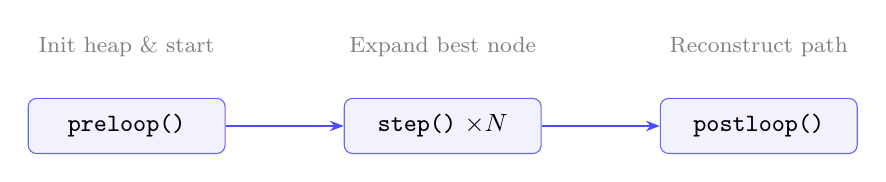
\begin{tikzpicture}[
  box/.style={rectangle, draw=blue!60, fill=blue!5, rounded corners=3pt,
              minimum width=2.5cm, minimum height=0.7cm, text centered, font=\small},
  arr/.style={-{Stealth[length=5pt]}, blue!70, thick}
]
\node[box] (pre)  {\texttt{preloop()}};
\node[box, right=1.5cm of pre]  (step) {\texttt{step()} $\times N$};
\node[box, right=1.5cm of step] (post) {\texttt{postloop()}};

\draw[arr] (pre) -- (step);
\draw[arr] (step) -- (post);

\node[above=0.4cm of pre,  font=\footnotesize, gray] {Init heap \& start};
\node[above=0.4cm of step, font=\footnotesize, gray] {Expand best node};
\node[above=0.4cm of post, font=\footnotesize, gray] {Reconstruct path};
\end{tikzpicture}
\end{center}

The \texttt{plan()} method in the base class calls these three hooks in order
up to \texttt{iter\_limit = 10000} iterations.
\texttt{AStarImplementation} overrides all three.

% ==============================================================================
\section{Path Smoothing}
% ==============================================================================

The raw A* path is jagged --- it follows grid diagonals and cardinal steps.
A smooth path is easier for a robot to follow and nicer to visualise.

\subsection{Adaptive Waypoint Downsampling}

The full A* path may contain hundreds of nodes. Before fitting a spline,
the path is downsampled to a small set of \textbf{representative waypoints}:

\begin{itemize}
  \item Corners (high curvature turns) --- kept at dense spacing.
  \item Straight segments --- kept at sparse spacing.
\end{itemize}

This balances faithfulness to the original path near obstacles with
smoothness on open stretches.

\subsection{Natural Cubic Spline}

A \textbf{natural cubic spline} is fit independently to the $x$ and $y$
coordinates of the waypoints, parameterised by cumulative arc length $s$:

\begin{tcolorbox}[formulabox, title={Cubic Spline Parameterisation}]
Given waypoints $(x_0, y_0), (x_1, y_1), \ldots, (x_k, y_k)$ with
cumulative arc lengths $s_0 = 0,\; s_i = s_{i-1} + \|(x_i - x_{i-1},\, y_i - y_{i-1})\|$:
\begin{align}
  x(s) &= \sum_{i} a^x_i s^3 + b^x_i s^2 + c^x_i s + d^x_i \\
  y(s) &= \sum_{i} a^y_i s^3 + b^y_i s^2 + c^y_i s + d^y_i
\end{align}
The natural boundary condition sets the second derivative to zero at
both endpoints: $x''(s_0) = x''(s_k) = 0$, ensuring the path
does not curve artificially at start or goal.
\end{tcolorbox}

The spline is then sampled at 300 evenly-spaced arc-length values to produce
the final \texttt{smooth\_path} list of \texttt{PathNode} objects published
on \texttt{smooth\_path}.

% ==============================================================================
\section{Pose Sources}
% ==============================================================================

\texttt{navigation\_node} supports two ways to receive the robot's current
position, selected by the \texttt{pose\_source} parameter.

\begin{center}
\begin{tabular}{llll}
\toprule
\textbf{pose\_source} & \textbf{Topic} & \textbf{Message} & \textbf{Use case} \\
\midrule
\texttt{"dummy"} & \texttt{current\_position} & \texttt{PointStamped} & Testing with a fake publisher \\
\texttt{"relocalization"} & \texttt{/relocalization/pose} & \texttt{Pose} & Live ORB-SLAM3 output \\
\bottomrule
\end{tabular}
\end{center}

\subsection{Dummy Mode}

In dummy mode the node subscribes to \texttt{current\_position}
(\texttt{geometry\_msgs/PointStamped}). The message uses \textbf{user space}
coordinates (Section~4): \texttt{point.x} is $X_u$ (upward), \texttt{point.y} is
$Y_u$ (rightward), with origin at bottom-left.

A test publisher (\texttt{position\_publisher.py}) shuttles a fake robot
between two waypoints at 10~Hz to allow end-to-end testing without a robot.

\subsection{Relocalization Mode}

In relocalization mode the node subscribes to
\texttt{/relocalization/pose} (\texttt{geometry\_msgs/Pose}).
The ORB-SLAM3 pose is in \textbf{world metres} and must be converted
to pixel coordinates using the map metadata received on \texttt{/map\_meta}:

\begin{lstlisting}[style=python, caption={World-to-pixel conversion in relocalization\_pose\_callback}]
col = int((msg.position.x - self._map_x_min) / self._map_resolution)
row = map_h - 1 - int((msg.position.z - self._map_z_min) / self._map_resolution)
col = max(0, min(map_w - 1, col))
row = max(0, min(map_h - 1, row))
current = PixelCoords(col, row)
\end{lstlisting}

\begin{tcolorbox}[warningbox, title={Common Mistake}]
  Using raw world coordinates without subtracting $(x_{\min}, z_{\min})$
  places the robot at pixel $(0,0)$ whenever it is near the ORB-SLAM3
  world origin $(0,0,0)$ --- which is almost certainly \emph{outside} the
  map extent. The A* planner will immediately reject this as a blocked
  start cell. Always subtract the map offsets.
\end{tcolorbox}

% ==============================================================================
\section{Deviation Detection and Replanning}
% ==============================================================================

The navigation node monitors whether the robot has strayed too far from the
planned path. If it has, it replans automatically from the robot's current
position.

\begin{tcolorbox}[formulabox, title={Deviation Check}]
Given the current robot pixel position $(r_x, r_y)$ and the set of smooth
path nodes $\mathcal{P}$:
\[
  d_{\min} = \min_{p \in \mathcal{P}}\; \sqrt{(p_x - r_x)^2 + (p_y - r_y)^2}
\]
If $d_{\min} > \tau$ (default $\tau = 5$~px), replanning is triggered.
\end{tcolorbox}

A threshold of 5~pixels at 0.02~m/px corresponds to 10~cm in the real world.
Replanning sets \texttt{start\_coords} to the current robot position and
calls \texttt{try\_plan()} which re-runs A* and redraws the path image.

% ==============================================================================
\section{Visualization Pipeline}
% ==============================================================================

The navigation node maintains three image layers and publishes each as a
separate ROS topic so different consumers can subscribe to the level of
detail they need.

\begin{center}
\begin{tabular}{lll}
\toprule
\textbf{Topic} & \textbf{Contents} & \textbf{Updated when} \\
\midrule
\texttt{static\_image}  & Raw occupancy grid only & New map arrives \\
\texttt{path\_image}    & Grid + planned path + start/goal markers & New plan computed \\
\texttt{trails\_image}  & Path image + robot trail + heading indicator & Every pose update \\
\bottomrule
\end{tabular}
\end{center}

\subsection{Trail}

The robot's position history is stored in a \texttt{deque(maxlen=500)}.
When rendered, the trail is drawn as a grey polyline using
\texttt{cv2.polylines}.

\subsection{Heading Indicator (Triangle)}

A cyan filled triangle indicates the robot's current heading.
The triangle tip points in the direction of motion.

\begin{tcolorbox}[formulabox, title={Heading Angle}]
The heading angle $\theta$ is computed from the robot's movement vector
over a \textbf{10-frame lookback window}:
\[
  (dx, dy) = (x_{\text{now}} - x_{t-10},\; y_{\text{now}} - y_{t-10})
\]
\[
  \theta = \mathrm{atan2}(dy,\, dx)
  \quad \text{(updated only if } dx^2 + dy^2 \geq 4\text{)}
\]
The minimum-distance guard ($\|{(dx,dy)}\| \geq 2$~px) prevents single-pixel
lateral noise from snapping the heading to left or right.
\end{tcolorbox}

The triangle is defined in local coordinates and rotated by $\theta$:

\begin{tcolorbox}[formulabox, title={Triangle Rotation}]
Local triangle vertices (tip forward along $+x$):
\[
  V_{\text{local}} = \begin{bmatrix} L & 0 \\ -L/2 & -W \\ -L/2 & W \end{bmatrix}
  \quad (L=9,\; W=4)
\]
Rotation matrix:
\[
  R(\theta) = \begin{bmatrix} \cos\theta & -\sin\theta \\ \sin\theta & \cos\theta \end{bmatrix}
\]
World vertices:
\[
  V = V_{\text{local}}\, R(\theta)^T + (c_x,\; c_y)
\]
where $(c_x, c_y)$ is the robot pixel position.
\end{tcolorbox}

\begin{tcolorbox}[notebox]
  The default heading at startup is $\theta = -\pi/2$ (pointing upward
  on screen). This means the triangle faces up even before the robot
  has accumulated enough trail to compute a direction.
\end{tcolorbox}

% ==============================================================================
\section{Configuration}
% ==============================================================================

Runtime parameters are set in
\texttt{src/navigation/navigation/config/navigation\_params.yaml}:

\begin{lstlisting}[style=yaml, caption={navigation\_params.yaml}]
navigation_node:
  ros__parameters:
    pose_source: "dummy"      # "dummy" | "relocalization"
    pose_scale:  1.0          # reserved; not used in current coordinate math
\end{lstlisting}

\begin{center}
\begin{tabular}{lll}
\toprule
\textbf{Parameter} & \textbf{Default} & \textbf{Effect} \\
\midrule
\texttt{pose\_source} & \texttt{"dummy"} &
  Subscribe to \texttt{current\_position} (PointStamped) or
  \texttt{/relocalization/pose} (Pose) \\
\texttt{pose\_scale}  & \texttt{1.0} & Multiplier reserved for future rescaling \\
\bottomrule
\end{tabular}
\end{center}

After changing the YAML, rebuild once to propagate the file to the install tree:

\begin{lstlisting}[style=yaml]
colcon build --symlink-install --packages-select navigation
source install/setup.bash
\end{lstlisting}

% ==============================================================================
\section{End-to-End Flowchart}
% ==============================================================================

\begin{figure}[h]
\centering
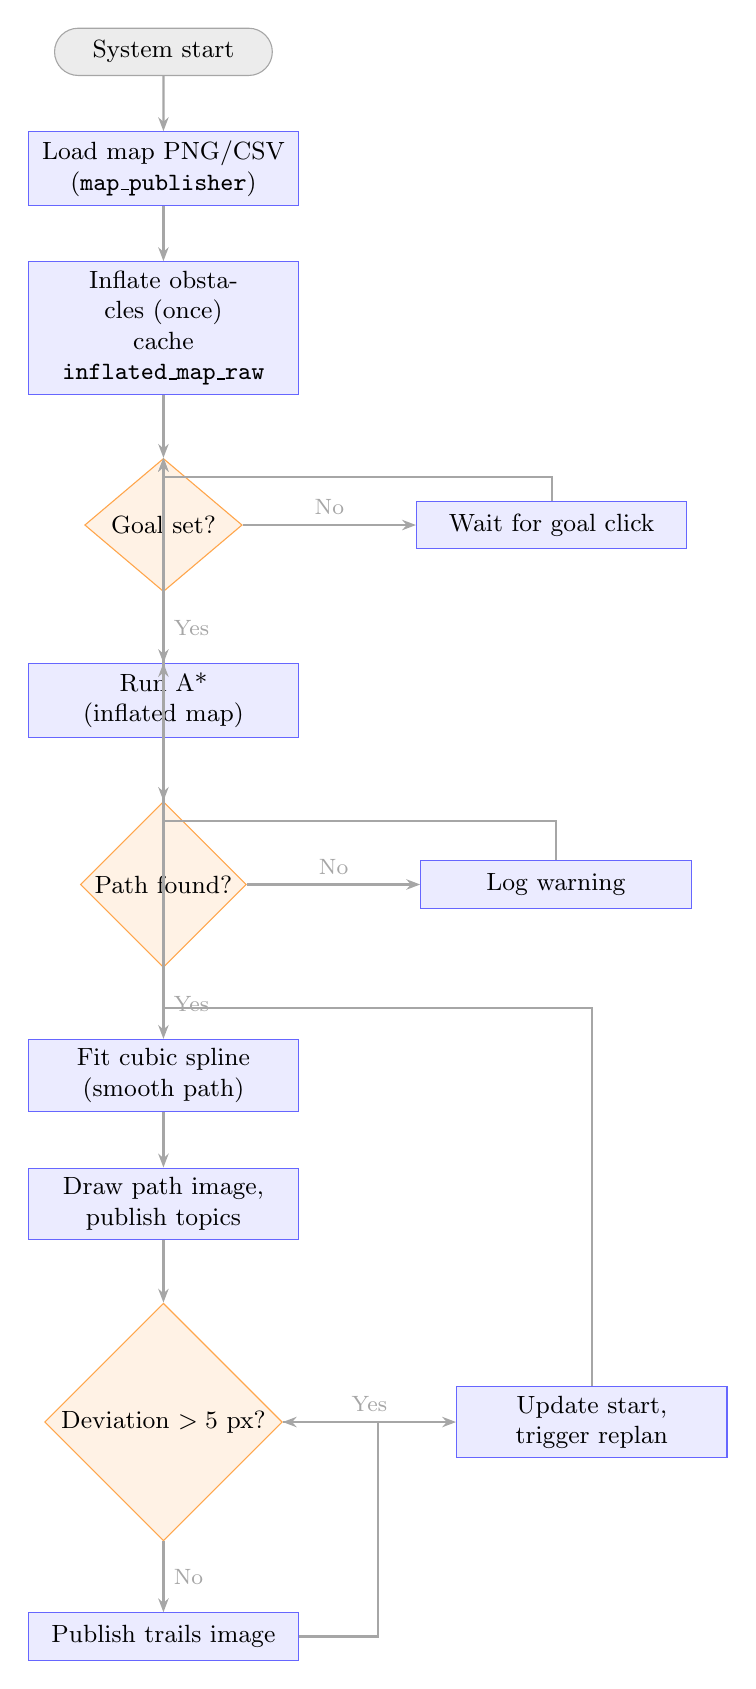
\begin{tikzpicture}[
  node distance=0.7cm and 2.5cm,
  startstop/.style={rounded rectangle, draw=gray!70, fill=gray!15,
                    minimum width=3cm, minimum height=0.6cm,
                    font=\small, text centered},
  process/.style={rectangle, draw=blue!60, fill=blue!8,
                  minimum width=3cm, minimum height=0.6cm,
                  font=\small, text centered, text width=3.2cm},
  decision/.style={diamond, draw=orange!70, fill=orange!10,
                   minimum width=2cm, minimum height=0.6cm,
                   font=\small, text centered, inner sep=1pt},
  arr/.style={-{Stealth[length=5pt]}, thick, gray!70},
]

\node[startstop] (start) {System start};
\node[process, below=of start] (loadmap) {Load map PNG/CSV\\(\texttt{map\_publisher})};
\node[process, below=of loadmap] (inflate) {Inflate obstacles (once)\\cache \texttt{inflated\_map\_raw}};
\node[decision, below=0.8cm of inflate] (havegoal) {Goal set?};
\node[process, right=2.2cm of havegoal] (wait) {Wait for goal click};
\node[process, below=0.9cm of havegoal] (plan) {Run A*\\(inflated map)};
\node[decision, below=0.8cm of plan] (planok) {Path found?};
\node[process, right=2.2cm of planok] (warn) {Log warning};
\node[process, below=0.9cm of planok] (smooth) {Fit cubic spline\\(smooth path)};
\node[process, below=of smooth] (draw) {Draw path image,\\publish topics};
\node[decision, below=0.8cm of draw] (deviate) {Deviation $> 5$~px?};
\node[process, right=2.2cm of deviate] (replan) {Update start,\\trigger replan};
\node[process, below=0.9cm of deviate] (trail) {Publish trails image};
\node[arr] (loopback) {};

\draw[arr] (start) -- (loadmap);
\draw[arr] (loadmap) -- (inflate);
\draw[arr] (inflate) -- (havegoal);
\draw[arr] (havegoal.east) -- (wait.west) node[midway,above,font=\footnotesize]{No};
\draw[arr] (wait.north) |- ++(0,0.3) -| (havegoal.north);
\draw[arr] (havegoal.south) -- (plan) node[midway,right,font=\footnotesize]{Yes};
\draw[arr] (plan) -- (planok);
\draw[arr] (planok.east) -- (warn.west) node[midway,above,font=\footnotesize]{No};
\draw[arr] (warn.north) |- ++(0,0.5) -| (havegoal.north);
\draw[arr] (planok.south) -- (smooth) node[midway,right,font=\footnotesize]{Yes};
\draw[arr] (smooth) -- (draw);
\draw[arr] (draw) -- (deviate);
\draw[arr] (deviate.east) -- (replan.west) node[midway,above,font=\footnotesize]{Yes};
\draw[arr] (replan.north) |- ++(0,4.8) -| (plan.north);
\draw[arr] (deviate.south) -- (trail) node[midway,right,font=\footnotesize]{No};
\draw[arr] (trail.east) -- ++(1.0,0) |- (deviate.east);

\end{tikzpicture}
\caption{End-to-end planning and visualization loop.}
\label{fig:flowchart}
\end{figure}

% ==============================================================================
\section{Key Takeaways}
% ==============================================================================

\begin{enumerate}[label=\textbf{\arabic*.}]

  \item \textbf{Inflate once, plan many times.}
        Obstacle inflation is the most expensive preprocessing step.
        By caching it after every map update and passing it directly to the
        planner, the system avoids re-inflating on every goal click or
        deviation replan.

  \item \textbf{Three coordinate systems, one internal representation.}
        All A* computation happens in pixel space (column, row).
        User clicks and ORB-SLAM3 poses are converted at the boundary,
        not inside the planner.

  \item \textbf{Map origin offset is not optional.}
        The occupancy grid shifts the world origin to its own bottom-left
        corner. Live poses \emph{must} subtract $(x_{\min}, z_{\min})$ before
        dividing by resolution, or the robot will appear at a wrong location.

  \item \textbf{Lazy deletion makes A* fast on large grids.}
        Pushing a new heap entry instead of updating an existing one reduces
        the per-relaxation cost from $O(n)$ (linear scan) to $O(\log n)$.
        On a 200$\times$200 grid this typically completes in under 5~ms.

  \item \textbf{Heading stability requires a look-back window.}
        Computing heading from just one previous trail point amplifies pixel-
        level noise. A 10-frame look-back with a 2-pixel minimum-movement
        guard produces a stable indicator that correctly reflects the robot's
        true direction of travel.

\end{enumerate}

\end{document}
